\documentclass[dvisvgm]{minimal}
\usepackage{tikz}

% Set font from website
\usepackage[T1]{fontenc}
\usepackage[default]{sourcesanspro}

% Set colors from website
\usepackage{xcolor}
\definecolor{qe-gray}{RGB}{68,68,68}
\definecolor{qe-blue}{RGB}{0, 114, 188}
\definecolor{blue}{rgb}{0.23,0.58,0.89}
\definecolor{green}{rgb}{0.24,0.64,0.30}

\begin{document}
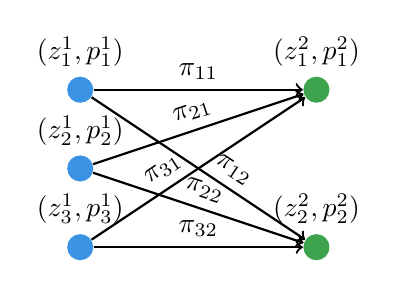
\begin{tikzpicture}
%		\draw[help lines] (0,0) grid (3,3);
\node[circle, fill= blue, label={$(z_1^1, p_1^1)$}] (1) at (0,2) {};
\node[circle, fill= blue, label={$(z_2^1, p_2^1)$}] (2) at (0,1) {};
\node[circle, fill= blue, label={$(z_3^1, p_3^1)$}] (3) at (0,0) {};
\node[circle, fill= green, label={$(z_1^2, p_1^2)$}] (4) at (3,2) {};
\node[circle, fill= green, label={$(z_2^2, p_2^2)$}] (5) at (3,0) {};
\draw[thick, ->] (1) edge node [sloped, above] {$\pi_{11}$} (4);
\draw[thick, ->] (2) edge node [sloped, above] {$\pi_{21}$} (4);
\draw[thick, ->] (3) edge node [sloped, above left] {$\pi_{31}$} (4);
\draw[thick, ->] (1) edge node [sloped, above right] {$\pi_{12}$} (5);
\draw[thick, ->] (2) edge node [sloped, above] {$\pi_{22}$} (5);
\draw[thick, ->] (3) edge node [sloped, above] {$\pi_{32}$} (5);
\end{tikzpicture}
\end{document}